\section{\qt}
\label{sec:qtip}

% \albert{add novel trellis coding section, section 4 is ``qtip''
% section 4 says we combine with incp from qs. 

% the stuff in the middle (how to round) is totally agnostic, for our experiments we use adaptive rounding, but you could do whatever aqlm does
% }

Quantizing with TCQ requires storing both the codebook ($2^L \times V$) and trellis structure ($2^L \times 2^{kV}$) during inference. 
These components are too large for fast inference when $L \gtrapprox 12$, which is necessary for high quality. 
Furthermore, for a generic trellis, recovering the state (and so the decoded value) at step $t$th requires a graph walk using the first $kt$ bits: this prevents parallel decoding. % neighboring groups in $\hat S$ have sequential dependencies that prevent parallel decoding.
\qts solves these problems with a novel combination of incoherence processing, a hardware-efficient ``bitshift trellis,'' and fast compute-based random Gaussian codes.
Incoherence processing makes $W$ approximatelly i.i.d Gaussian, which reduces quantization to Gaussian source coding.
The bitshift trellis removes needing to store the trellis structure during decoding and also enables parallel decoding.
Finally, the fast compute-based random Gaussian codes remove the need to store the full codebook, completing the equation for fast inference.
On the quality side, the fast random Gaussian codes enable the simple bitshift trellis to match complicated trellises and achieve \sota quantization quality.

The main focus of \qts is on \textit{what to quantize with} (i.e.\ TCQ) and not \textit{how to quantize} (e.g.\ adaptive rounding or descent methods).
The general construction of \qts can be used as a drop-in replacement for VQ in any rounding framework.
In the following sections, we first describe the ``bitshift'' trellis (Section \ref{sec:bitshift}). 
Then, we describe a series of fast compute-based codes for i.i.d Gaussian sources, aligning with different types of hardware (Sections \ref{sec:computed} and \ref{sec:hybrid}).
Finally, we give an approximation for the tail-biting trellis problem, which lets us more efficiently load weights in hardware (Section \ref{sec:tailbiting}).


% \qts has two main steps.
% First, we perform incoherence processing to make $W$ approximately i.i.d Gaussian.
% Then, we perform TCQ with the ``bitshift'' trellis and fast hybrid and computed Gaussian codes to enable fast inference.
% Since the proxy error is not an additive distortion metric, we cannot minimize it by quantizing $W$ as one sequence.
% Instead, we use TCQ as a quantizer in BlockLDLQ, which allows us to simultaneously achieve high dimensionality and low proxy error.
% Specifically, we quantize a block of $T_x \times T_y$ weights as a sequence, where $T_x$ and $T_y$ span the output and input dimensions of $W$, respectively.
% Since BlockLDLQ only specifies feedback along the input dimension, this mathematically equivalent to BlockLDLQ with $g=T_y$ but a vector dimension of $T_xT_y \gg T_y$. 
% We note that while we use TCQ within BlockLDLQ, one could use our construction of TCQ as a drop-in replacement for VQ in any situation with an i.i.d source.

\subsection{``Bitshift'' Trellis and Codebook Design}
\label{sec:bitshift}


\begin{figure}[t]
\centering
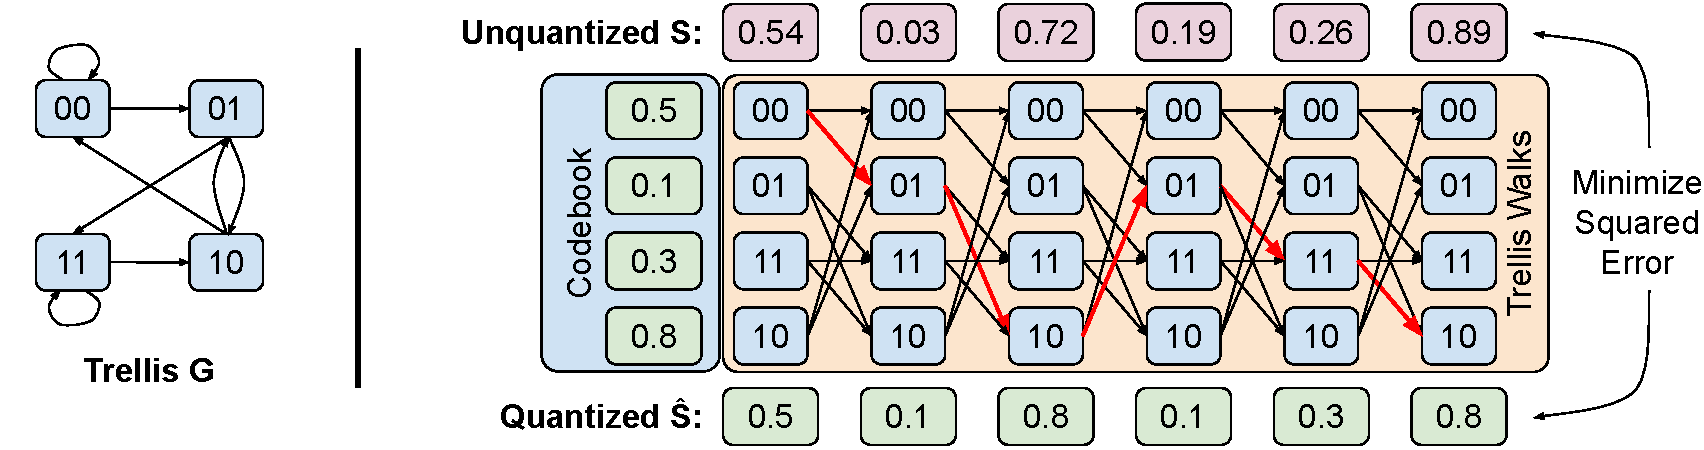
\includegraphics[width=\linewidth]{images/bitshift_trellis.pdf}
\caption{A bitshift trellis code with $L = 2, k = 1, V = 1$. Nodes 0, 1, 2, and 3 have code values 0.5, 0.1, 0.8, and 0.3, respectively. Each node can only transition to the $2^{kV} = 2$ nodes that share their top $L-kV = 1$ bit with its bottom $L-kV = 1$ bit. In this example, $\hat S$ can be stored as \texttt{0010110}. $\hat S$ is also \textit{tail-biting}, so the last $L-kV = 1$ bits can be dropped to give $\hat S =$ \texttt{001011}.}
\label{fig:bitshift}
\end{figure}

The bitshift trellis was introduced by \citet{rptc} as part of the ``random permutation trellis coder'' (RPTC). 
In the bitshift trellis, node $i$ has an edge to node $j$ if $\exists c\in \mathbb{Z}, 0 \le c < 2^{kV},$ s.t. $j = (i2^{kV} \mbox{ mod } 2^L) + c$. 
Essentially, the top $L-kV$ bits of $j$ equal the bottom $L-kV$ bits of $i$.
This means that the first group of $V$ weights depends only on the bits at positions $\{ 1, 2, \ldots, L \}$, the second only on bit positions $\{kV+1, kV+2, \ldots, kV+L\}$, and in general the $t$th on bit positions $\{(t-1)kV+1, \ldots, (t-1)kV+L\}$.
During inference, obtaining the next compressed group of $V$ weights in a sequence only requires bitshifting by $kV$ bits, which is supported on virtually all hardware.
Furthermore, since each group of $V$ weights only depends on a contiguous window of $L$ bits in $\hat S$, decoding can be parallelized.
Figure \ref{fig:bitshift} shows a simple $(L=2, k=1, V=1)$ bitshift trellis. 
Note that edges only exist between nodes that overlap by 1 bit, and storing the quantized length 6 $\hat S$ indeed only requires 6 bits (plus the initial state).

Quantizing an i.i.d.\ source with the bitshift trellis is nontrivial because neighboring groups of weights sharing many bits can potentially lead to strong correlations (Figure \ref{fig:corr} LL).
The RPTC permutes the codebook to decorrelate neighboring weight groups (Figure \ref{fig:corr} RR) \cite{rptc}.
However, this requires storing the codebook or storing and applying the permutation, both of which are prohibitively expensive during decoding.
Instead, \qts introduces a series of compute-based codes to produce a psuedorandom code, which has the same decorrelating effect and admits fast inference.
To match approximately i.i.d.\ Gaussian RHT-transformed matrices, these codes produce psuedorandom approximate Gaussians in as few as 2 instructions per weight (see Table \ref{tab:distortion} and Figure \ref{fig:corr}).
To the best of our knowledge, these code constructions alone are novel and we are the first to propose a lookup-free Gaussian trellis code.


\begin{table}[t]
\caption{\qt's compute-based codes (1MAD, 3INST, HYB) achieve similar distortion rates as a pure-lookup random Gaussian trellis code (RPTC) when quantizing an i.i.d Gaussian source to 2 bits. All TCQ methods ($L=16$) outperform SQ and VQ and are significantly closer to the infinite-length distortion rate $D_R$, which lower bounds the distortion a $k$-bit quantizer can attain.} 
\centering
\sc\small
\begin{tabular}{ccccccccc}
                            &             SQ                   &              VQ                 & \multicolumn{3}{c}{1D TCQ}                 & \multicolumn{2}{c}{2D TCQ}         &          \\ \hline
\multicolumn{1}{c|}{Quant.} & \multicolumn{1}{c|}{Lloyd-Max} & \multicolumn{1}{c|}{\qss E8P} & 1MAD  & 3INST & \multicolumn{1}{c|}{RPTC}  & HYB   & \multicolumn{1}{c|}{RPTC}  & $D_R$      \\ \hline
\multicolumn{1}{c|}{Dim.}   & \multicolumn{1}{c|}{1}         & \multicolumn{1}{c|}{8}        & 256   & 256   & \multicolumn{1}{c|}{256}   & 256   & \multicolumn{1}{c|}{256}   & $\infty$ \\
\multicolumn{1}{c|}{MSE.}   & \multicolumn{1}{c|}{0.118}      & \multicolumn{1}{c|}{0.089}     & 0.069 & 0.069 & \multicolumn{1}{c|}{0.068} & 0.071 & \multicolumn{1}{c|}{0.069} & 0.063    \\ \hline
\end{tabular}
\label{tab:distortion}
\end{table}

%\qingyao{We should move subsections 3.2.1 and 3.2.2 to the Appendix, as they provide little extra information when we already have the pseudocode.}
%\albert{no, nobody is going to understand the pseudocode without an explanation}
%\albert{rewrite this part to reflect what was written in the tcq section above}
% Naively choosing a codebook such as $\mbox{state\ } i \gets \mbox{icdf}(\frac{i+1}{2^L + 1})$, where icdf is the standard Gaussian inverse CDF, results in strong correlations and poor quantization quality; this is because neighboring weights $w_iw_{i+1}$ share $L-kV$ bits.
% Mao et al. solve this by applying a fixed permutation $\pi$ to the $L$ bits representing a weight, which decorrelates neighboring weights.
% However, this requires a permutation during inference, which is expensive.
% Instead, we note that permuting \textit{the codebook} has the same decorrelating effect, which reduces the codebook design problem to finding a random Gaussian codebook. 
\subsubsection{Lookup-Free Computed Codes}
\label{sec:computed}

\begin{figure}[t]
\centering
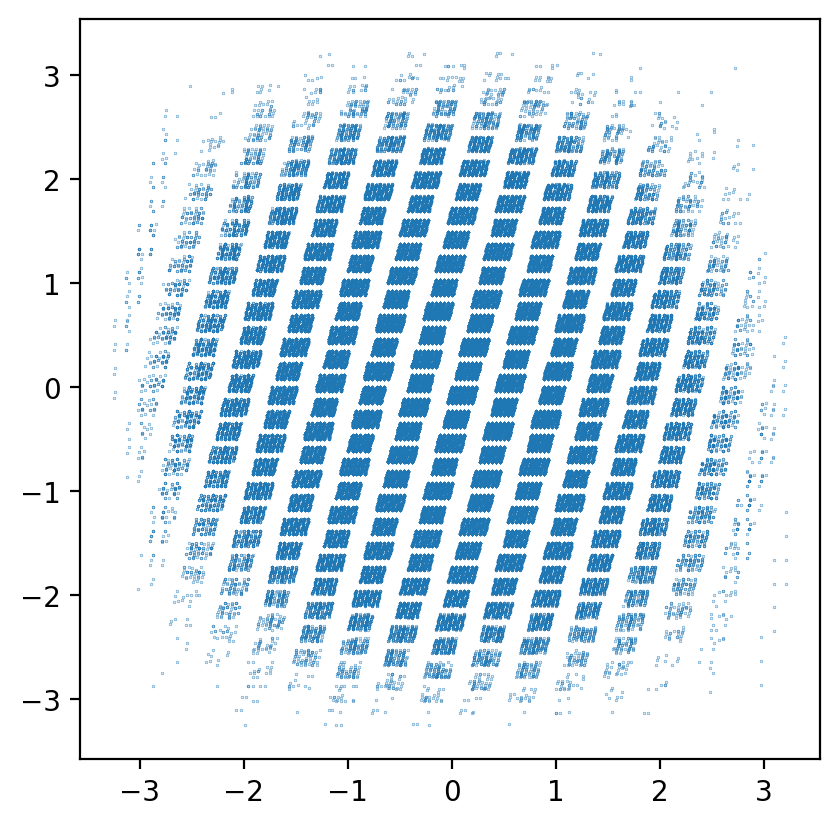
\includegraphics[width=0.24\linewidth]{images/bad_corr.png}
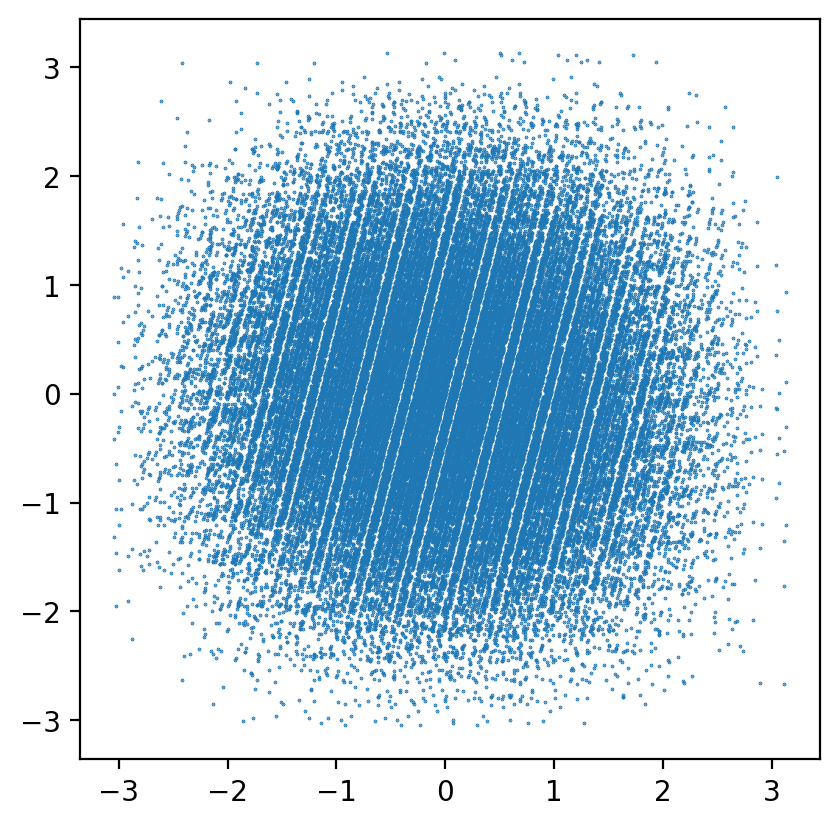
\includegraphics[width=0.24\linewidth]{images/1mad.png}
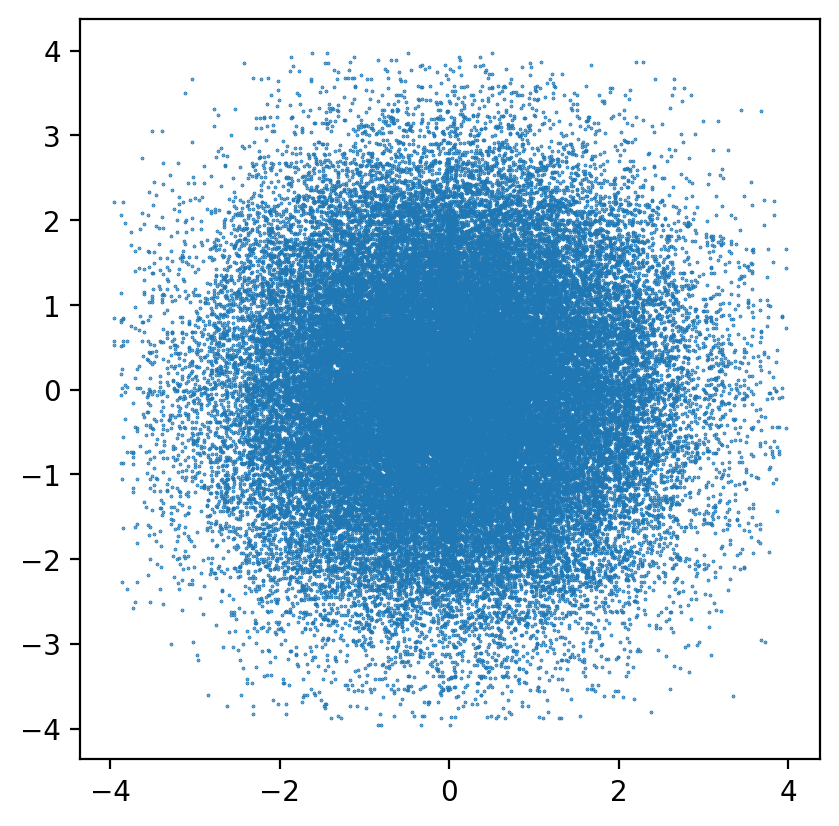
\includegraphics[width=0.24\linewidth]{images/3inst.png}
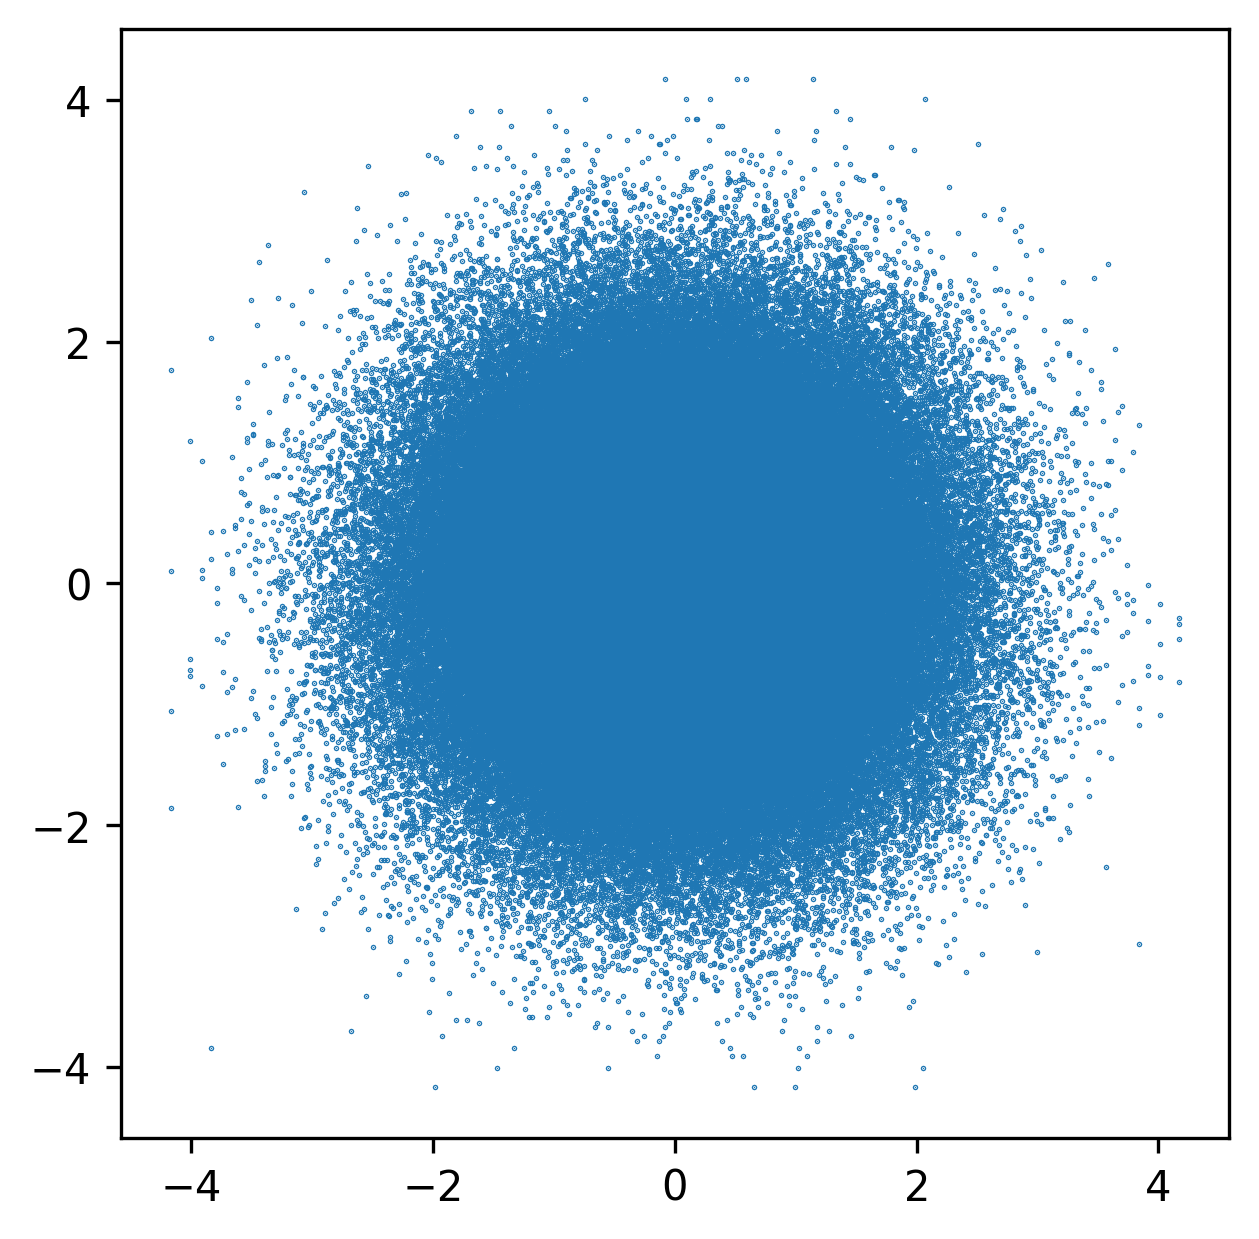
\includegraphics[width=0.24\linewidth]{images/rptc.png}
\caption{Set of representable neighboring values in a bitshift trellis with $L=16, k=2, V=1$ for (far left) a code with strong correlations, (left center) algorithm \ref{alg:1mad} (``1MAD''), (right center) algorithm \ref{alg:3inst} (``3INST''), and (far right) a random Gaussian code. Note that while 1MAD has minor correlations, both 1MAD and 3INST are close to a random Gaussian, resulting in good quantization quality.}
\label{fig:corr}
\end{figure}

Here, we present two pure-computed lookup-free codes that produce a pseudorandom approximately Gaussian number from a $L$ bit word, enabling fast decoding on cache-limited hardware.
These codes avoid strong correlations and can be implemented in $\le4$ hardware instructions per weight on NVIDIA GPUs. 
We present two codes here to illustrate that multiple such codes are possible: in practice a lookup-free code can be designed to use the instructions available on whatever hardware we want to run on.

Algorithm \ref{alg:1mad} (1MAD) first runs a linear congruential generator (LCG) to produce a pseudorandom 32-bit word \cite{lcg}.
This requires 2 instructions (\texttt{MAD} and \texttt{\&}). 
It then sums the 32-bit word as four 8-bit unsigned integers; this sum is approximately Gaussian distributed.
This requires 1 instruction (\texttt{vabsdiff4}).
Finally, this sum must be scaled and shifted (another \texttt{MAD}).
Although there are only $2^{10}$ representable values even when $L > 10$, this does not empirically affect quantization quality.
1MAD requires choosing $a$ and $b$ to avoid strong correlations; we set $a = 34038481$ and $b = 76625530$ (Figure \ref{fig:corr} LC).
%One can also further reduce correlations by adding a second LCG step.

Algorithm \ref{alg:3inst} (3INST) also first runs an LCG to produce a random 32-bit word $X$.
Then, it XORs the bottom 16 bits of $X$ with the mantissa bits, bottom two exponent bits, and sign bit of a magic FP16 number $m$ to produce an FP16 number $m_1$.
It then repeats this with the top 16 bits of $X$ to produce $m_2$ and returns $m_1 + m_2$. 
This entire process can be implemented in 3 ALU instructions\footnote{As there is currently no instruction on NVIDIA GPUs that sums the top and bottom half of a 32-bit word as two FP16s, this requires an extra data movement instruction to ``split'' the 32-bit word into two 16-bit registers.} with a \texttt{MAD} for the LCG, a \texttt{lop3} to mask and XOR with a packed duplicated $m$, and then summing $m_1$ and $m_2$.
$m_1 + m_2$ is approximately distributed by the sum of two mirrored exponential distributions, which is close to Gaussian.
Like with Algorithm \ref{alg:1mad}, $a, b,$ and $m$ must be chosen to avoid correlations; we used $a = 89226354, b = 64248484, m = 0.922$ (Figure \ref{fig:corr} right).

\begin{algorithm}[t]
\caption{Computed Gaussian Code ``1MAD''}
\begin{algorithmic}
\INPUT $L$-bit 0 left-padded integer $x$, \texttt{uint32} $a, b$.
\STATE $x \gets (ax+b) \mbox{\ mod\ } 2^{32}$ \COMMENT{run LCG to get uniform random $x$}

\COMMENT{sum $x$ as four 8-bit unsigned integers, this is approximately Gaussian}
\STATE $x \gets (x \verb| & | 255) + ((x \verb| >> | 8) \verb| & | 255) + ((x \verb| >> | 16) \verb| & | 255) + ((x \verb| >> | 24) \verb| & | 255)$ 
\STATE $x \gets (x - 510) / 147.8$
\OUTPUT Pseudorandom approximate Gaussian $x$.
\end{algorithmic}
\label{alg:1mad}
\end{algorithm}

\begin{algorithm}[t]
\caption{Computed Gaussian Code ``3INST''}
\begin{algorithmic}
\INPUT $L$-bit 0 left-padded integer $x$, \texttt{uint32} $a, b$, \texttt{float16} $m$.
\STATE $x \gets (ax+b) \mbox{\ mod\ } 2^{32}$ \COMMENT{run LCG to get uniform random $x$}

\COMMENT{modify sign, mantissa, and bottom 2 exponent bits of $m$ and sum, this is approximately Gaussian}
\STATE $m \gets \verb|reinterpret|(m, \verb|uint32|)$ \verb| << 16 | + \verb|reinterpret|(m, \verb|uint32|)
\STATE $x \gets (x \verb| & b10001111111111111000111111111111|) \verb| XOR | m$
\STATE $x \gets \verb|reinterpret|(x \verb| & | 2^{16} - 1, \verb|float16|) + \verb|reinterpret|((x \verb| >> | 16) \verb| & | 2^{16} - 1, \verb|float16|)$
\OUTPUT Pseudorandom approximate Gaussian $x$.
\end{algorithmic}
\label{alg:3inst}
\end{algorithm}

\subsubsection{Hybrid Lookup-Computed Codes}
\label{sec:hybrid}
Here, we describe a hybrid computed-lookup code that computes a pseudorandom (or hashed) index into a 2D vector codebook ($V=2$).
This code is tailored for modern GPUs, which have enough cache for a small in-memory LUT---one benefit of using such a LUT over a purely computed codebook is that a LUT can be fine-tuned after quantization. 
Algorithm \ref{alg:hyb} first performs the hash $X \gets X^2 + X$ to mix the lower order and upper order bits of $X$~\cite{klimov2003new}.
Then, it takes bits $(14-Q+1) - 14$ (0 indexed) as an index into a $2^Q \times 2$ LUT to get two 16-bit floats. (The reason why we chose a 2D codebook here is that shared memory on NVIDIA GPUs is accessed in 32-bit-word elements, and each such word can contain two 16-bit floats.)
Finally, it XORs bit 15 of $X$ to flip the sign of the second entry of the codebook vector.
Algorithm \ref{alg:hyb} can be implemented with \texttt{MAD}, bitshift, mask, and \texttt{lop3}, giving an amortized 2 instructions per weight.
This effectively assigns a $L$ bit word to one of $2^{Q+1}$ 2D vectors, each of which can be fine-tuned to improve quality.
Algorithm \ref{alg:hyb} can also be implemented to XOR bit 31 alongside bit 15 (this is free in the \texttt{lop3}) to give an effectively $2^{Q+2}$-sized codebook, which can improve quantization quality. 
We only realized this after running all the experiments, so the numbers in this paper use the ``one sign flip'' version of Algorithm \ref{alg:hyb}.
In \qt, we initialize the LUT using K-means on an empirical 2D i.i.d.\ Gaussian distribution.
%However, note that the lookup portion of this code can be initialized to any symmetric distribution, since the computation just performs an index hash.
%This means that this code can be used to quantize any i.i.d source.

\begin{algorithm}[t]
\caption{Hybrid Computed-Lookup 2D Gaussian Code ``HYB''}
\begin{algorithmic}
\INPUT $L$-bit 0 left-padded integer $x$, codebook $C \in \mathbb{R}^{2^{Q} \times (V=2)}$.
\STATE $x \gets x \cdot x + x \mbox{\ mod\ } 2^{32}$ \COMMENT{calculate hash}
\STATE $v \in \mathbb{R}^2 \gets C[(x \verb| >> | (15 - Q)) \verb| & | 2^Q - 1]$ \COMMENT{lookup from symmetric codebook}
\STATE $v \gets v \verb| XOR | (x \verb| & |(1 \verb| << | 15))$ \COMMENT{apply sign flip}
\OUTPUT Pseudorandom approximate Gaussian vector $v$.
\end{algorithmic}
\label{alg:hyb}
\end{algorithm}

\subsection{Tail-Biting Trellises}
\label{sec:tailbiting}
Directly quantizing a length-$T$ sequence to a $(L, k, V)$ trellis results in a total of $kT + L - kV$ bits since the starting state takes an additional $L-kV$ bits to store.
If we run inference on a machine with $w$-bit words where $w \vert kT$, we must read an extra $\lceil \frac{L - kV}{w} \rceil w - (L - kV)$ wasted bits per sequence.
For common $w$ (e.g. 32), setting $L = kV + w$ makes the Viterbi algorithm intractable.
One way to solve this is by enforcing that the start and end state share $L-kV$ bits, i.e. the trellis is \textit{tail-biting} \cite{771145}.
Exactly solving the tail-biting trellis problem via dynamic programming takes time quadratic in the state space ($2^L$), making this problem intractable for reasonable $L \ge 12$ \cite{ShaoRose1999TailBT}.
However, since RHT-processed weights are approximately i.i.d., simple algorithms can be effective for approximately solving the tail-biting problem. % the tail-biting overlap.
We propose Algorithm \ref{alg:tailbiting}, which first rotates the sequence by $T/2$, quantizes it, and then extracts the overlap between the rotated start and end states. 
It then requantizes the original sequence with this overlap as the tail-biting overlap.
This only requires two Viterbi calls in total.
Table \ref{tab:tailbiting} shows that in practice, Algorithm \ref{alg:tailbiting} can find close-to-optimal tail-biting sequences while being significantly cheaper to run than other tail-biting approximation algorithms \cite{ShaoRose1999TailBT}.


\begin{table}[t]
\vspace{-0.1cm}
\begin{tabular}{ll}
\centering
\begin{minipage}{0.48\textwidth}
\begin{algorithm}[H]
\caption{Tail-biting Trellis Approx.}
\begin{algorithmic}
\INPUT Sequence $S \in \mathbb{R}^T$, $(L, k, V)$ Trellis $G$.
\STATE $S' \gets $ Rotate $S$ to the right by $\lfloor T / 2 \rfloor$
\STATE $\hat S' \gets $ Viterbi($S'$, $G$)
\STATE $O \gets L-kV$ bit overlap of $\hat S'_{\lfloor T/2 \rfloor}\hat S'_{\lfloor T/2 \rfloor + 1}$
\STATE $\hat S \gets $ Viterbi($S$, $G$) with start/end overlap $= O$
\OUTPUT Tail biting $\hat S$
\end{algorithmic}
\label{alg:tailbiting}
\end{algorithm}
\end{minipage}
& 
\begin{minipage}{0.45\textwidth}
\centering
\caption{Quantizing 4K $T=256$ i.i.d Gaussian seqs. with a tail-biting $(12, k, 1)$ trellis.}
\vspace{-0.1cm}
%\sc\small
%\renewcommand{\arraystretch}{0.95}
\begin{tabular}{@{}ccc@{}}
\toprule
$k$ & Alg. \ref{alg:tailbiting} MSE & Optimal MSE \\ \midrule
1   & 0.2803           & 0.2798     \\
2   & 0.0733           & 0.0733     \\
3   & 0.0198           & 0.0198     \\
4   & 0.0055           & 0.0055     \\ \bottomrule
\end{tabular}
\label{tab:tailbiting}
\vspace{-0.4cm}
\end{minipage}
\end{tabular}
\end{table} 

